\documentclass[a4paper,10pt]{article}
\usepackage[utf8x]{inputenc}
\usepackage[top=1.5cm, bottom=1.5cm,left=2cm,right=1.5cm]{geometry}
%\usepackage{url}
\usepackage{listings}

%opening
\title{Statistical Analysis of ISMB 2012 Coverage at Twitter}
\author{Neil Saunders}

\usepackage{Sweave}
\begin{document}
\lstset{breaklines=true}
\Sconcordance{concordance:ismb.tex:ismb.Rnw:%
1 10 1 1 0 7 1 1 2 1 0 6 1 3 0 1 2 3 1 1 2 1 0 2 1 1 2 5 0 1 2 5 1 1 2 %
1 0 3 1 1 6 9 0 1 2 5 1 1 2 1 0 6 1 3 0 1 2 2 1 1 2 1 0 1 1 1 2 5 0 1 2 %
7 1 1 2 1 0 3 1 1 2 5 0 1 2 7 1 1 2 1 0 1 1 1 2 5 0 1 2 7 1 1 2 1 0 1 1 %
1 2 5 0 1 2 7 1 1 2 1 0 1 1 1 2 5 0 1 2 8 1 1 2 1 0 2 1 1 2 5 0 1 2 2 1 %
1 2 21 0 1 2 5 1 1 2 1 0 8 1 25 0 1 2 2 1 1 2 1 0 1 2 5 0 1 2 6 1 1 2 1 %
0 1 1 21 0 1 2 7 1 1 2 1 0 1 1 18 0 1 2 11 1}

\maketitle

\section{Preamble}
Load required libraries and data.
%load data
\begin{Schunk}
\begin{Sinput}
> library(ggplot2)
> library(xtable)
> library(RColorBrewer)
> library(tm)
> library(wordcloud)
> library(sentiment)
> load("../../data/ismb.RData")
\end{Sinput}
\end{Schunk}

\section{Tweets per day}
\begin{center}
\setkeys{Gin}{width=0.6\textwidth}
\begin{Schunk}
\begin{Sinput}
> ismb$date <- as.Date(ismb$created)
> byDay <- as.data.frame(table(ismb$date))
> colnames(byDay) <- c("date", "tweets")
> print(ggplot(byDay) + geom_bar(aes(date, tweets), fill = "salmon") + theme_bw()
+       + opts(title = "ISMB 2012 tweets per day"))
\end{Sinput}
\end{Schunk}
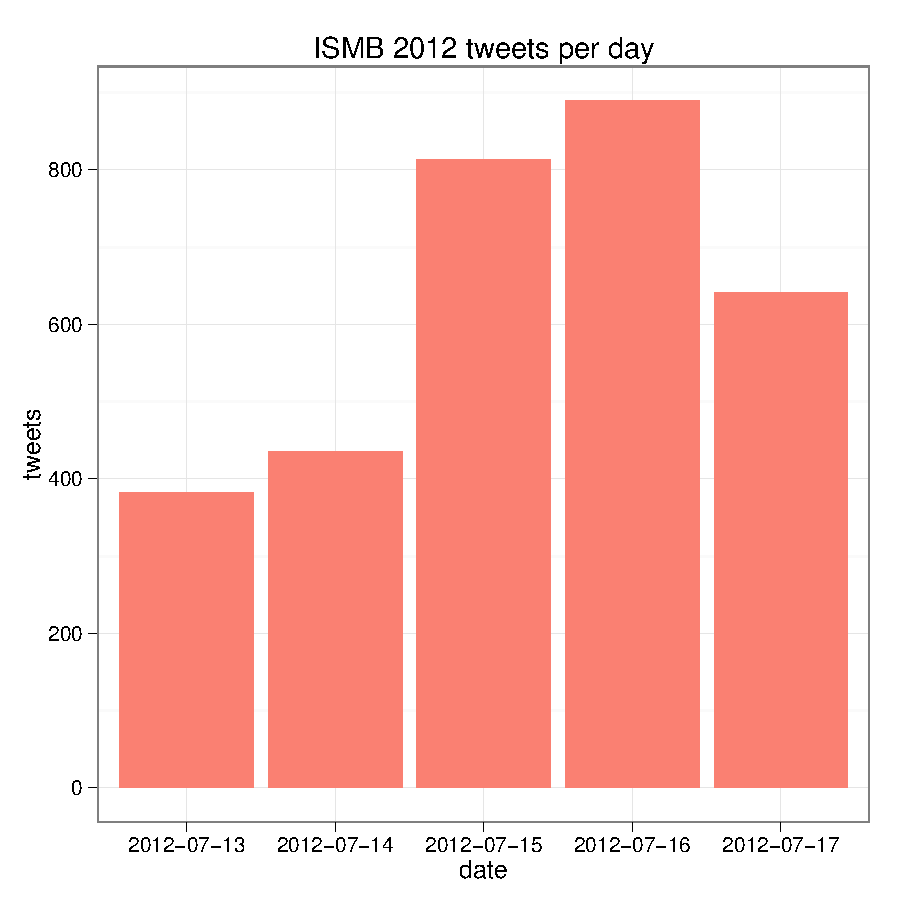
\includegraphics{ismb-002}
\end{center}

\newpage

\section{Tweets per hour by day}
\begin{center}
\begin{Schunk}
\begin{Sinput}
> ismb$hour <- as.POSIXlt(ismb$created)$hour
> byDayHour <- as.data.frame(table(ismb$date, ismb$hour))
> colnames(byDayHour) <- c("date", "hour", "tweets")
> byDayHour$hour <- as.numeric(as.character(byDayHour$hour))
> print(ggplot(byDayHour) + geom_bar(aes(hour, tweets), fill = "salmon", binwidth = 1) + 
+   facet_grid(date ~ hour) + 
+   opts(axis.text.x = theme_blank(), 
+        axis.ticks  = theme_blank(), 
+        panel.background = theme_blank(),
+        title = "ISMB 2012 tweets per hour by day"))
\end{Sinput}
\end{Schunk}
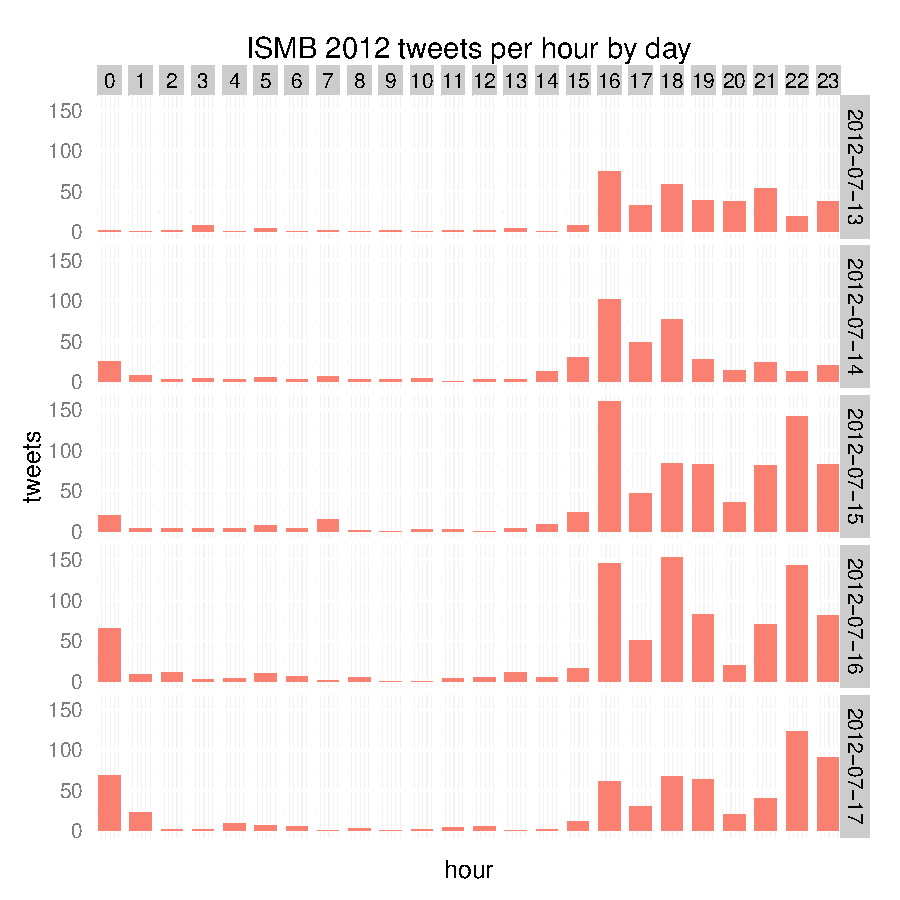
\includegraphics{ismb-003}
\end{center}

\newpage

\section{Popular talks}
First, get the hashtags:
\begin{Schunk}
\begin{Sinput}
> words <- strsplit(ismb$text, " ")
> hashtags <- lapply(words, function(x) x[grep("^#", x)])
> hashtags <- unlist(hashtags)
> hashtags <- tolower(hashtags)
> hashtags <- gsub("[^A-Za-z0-9]", "", hashtags)
> ht <- as.data.frame(table(hashtags))
> ht <- ht[sort.list(ht$Freq, decreasing=F),]
\end{Sinput}
\end{Schunk}

\subsection{Keynotes}
\begin{center}
\begin{Schunk}
\begin{Sinput}
> kn <- ht[grep("^kn", ht$hashtags),]
> kn$hashtags <- factor(kn$hashtags, levels = as.character(kn$hashtags))
> print(ggplot(tail(kn)) + geom_bar(aes(hashtags, Freq), fill = "salmon") + 
+   coord_flip() + theme_bw() + opts(title = "ISMB 2012 tweets - keynotes"))
\end{Sinput}
\end{Schunk}
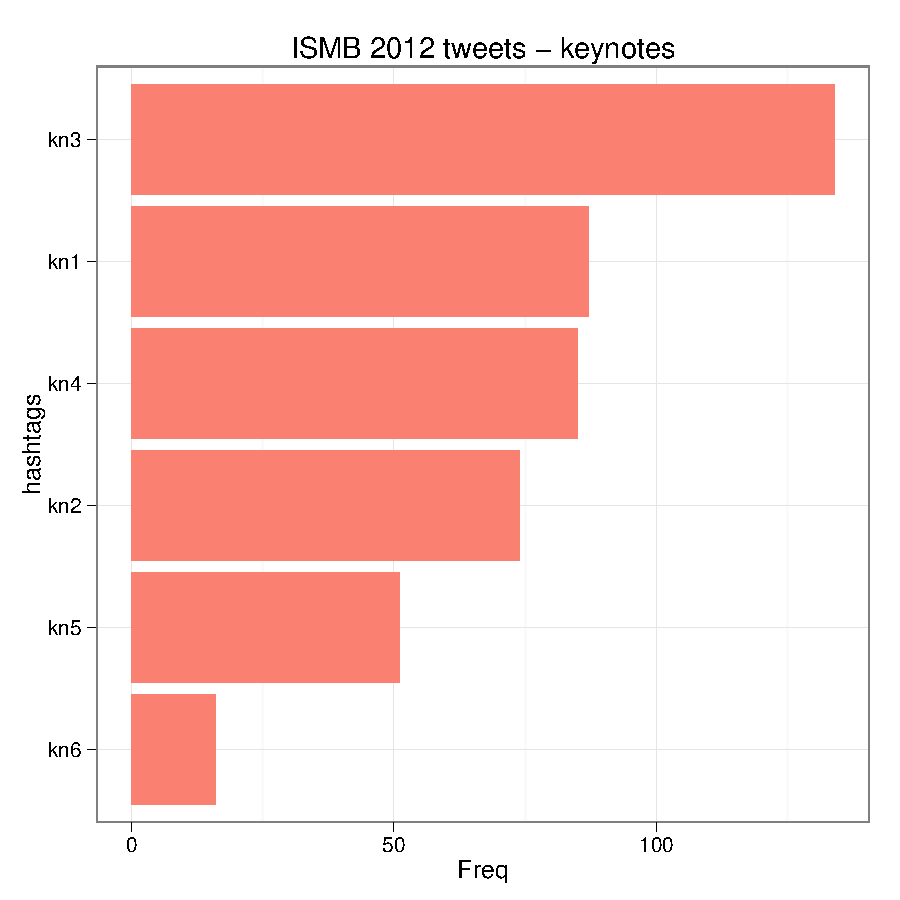
\includegraphics{ismb-005}
\end{center}

KN 3: Analysis of transcriptome structure and chromatin landscapes (Barbara Wold).

\newpage

\subsection{Published Papers}
\begin{center}
\begin{Schunk}
\begin{Sinput}
> pp <- ht[grep("^pp", ht$hashtags),]
> pp[47,2] <- 39
> pp <- pp[-5,]
> pp$hashtags <- factor(pp$hashtags, levels = as.character(pp$hashtags))
> print(ggplot(tail(pp, 20)) + geom_bar(aes(hashtags, Freq), fill = "salmon") + 
+   coord_flip() + theme_bw() + opts(title = "ISMB 2012 tweets - published papers"))
\end{Sinput}
\end{Schunk}
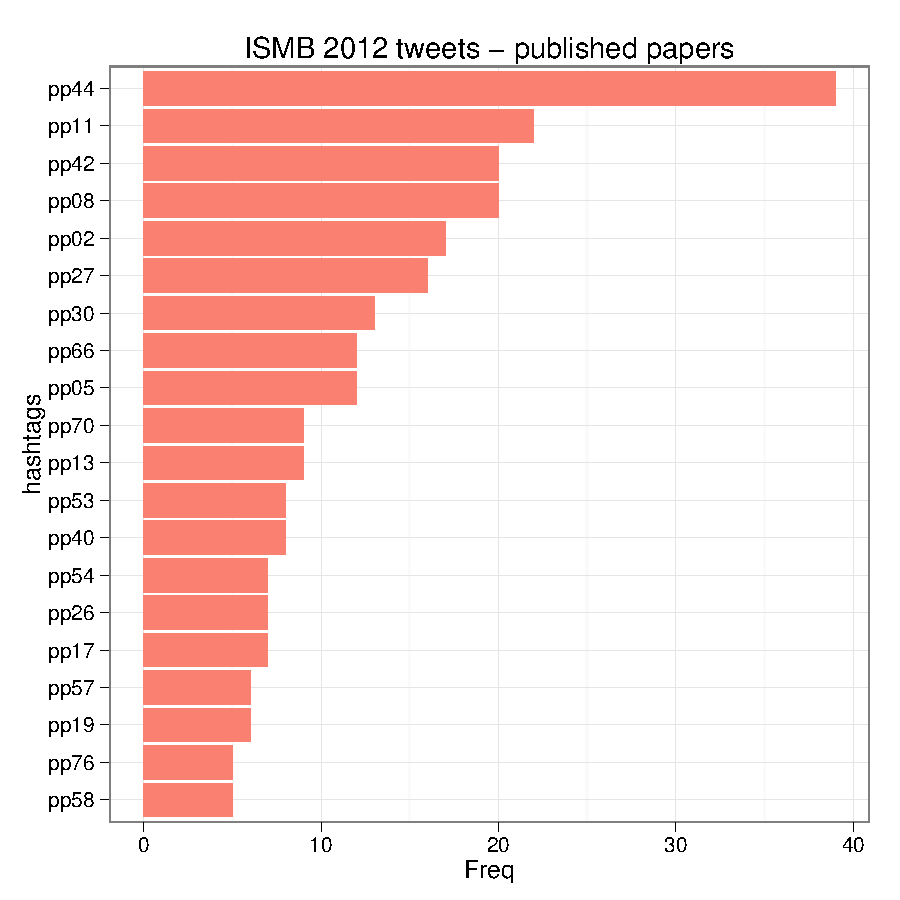
\includegraphics{ismb-006}
\end{center}

PP 44: Toward interoperable bioscience data (Susanna-Assunta Sansone).

\newpage

\subsection{Special Sessions}
\begin{center}
\begin{Schunk}
\begin{Sinput}
> ss <- ht[grep("^ss", ht$hashtags),]
> ss$hashtags <- factor(ss$hashtags, levels = as.character(ss$hashtags))
> print(ggplot(ss) + geom_bar(aes(hashtags, Freq), fill = "salmon") + 
+   coord_flip() + theme_bw() + opts(title = "ISMB 2012 tweets - special sessions"))
\end{Sinput}
\end{Schunk}
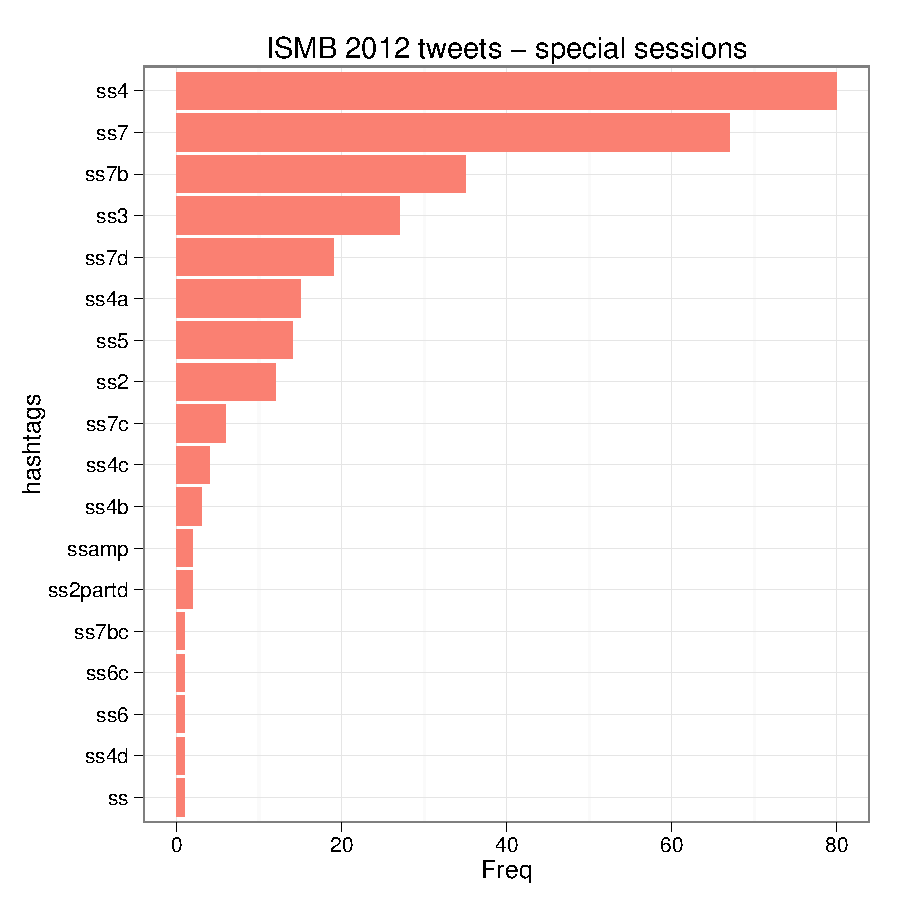
\includegraphics{ismb-007}
\end{center}

SS 4: Bioinformatic Integration of Diverse Experimental Data Sources (Kyle Ellrott,  David Haussler, Artem Sokolov, Josh Stuart).

\newpage

\subsection{Technology Track}
\begin{center}
\begin{Schunk}
\begin{Sinput}
> tt <- ht[grep("^tt", ht$hashtags),]
> tt$hashtags <- factor(tt$hashtags, levels = as.character(tt$hashtags))
> print(ggplot(tail(tt, 20)) + geom_bar(aes(hashtags, Freq), fill = "salmon") + 
+   coord_flip() + theme_bw() + opts(title = "ISMB 2012 tweets - technology track"))
\end{Sinput}
\end{Schunk}
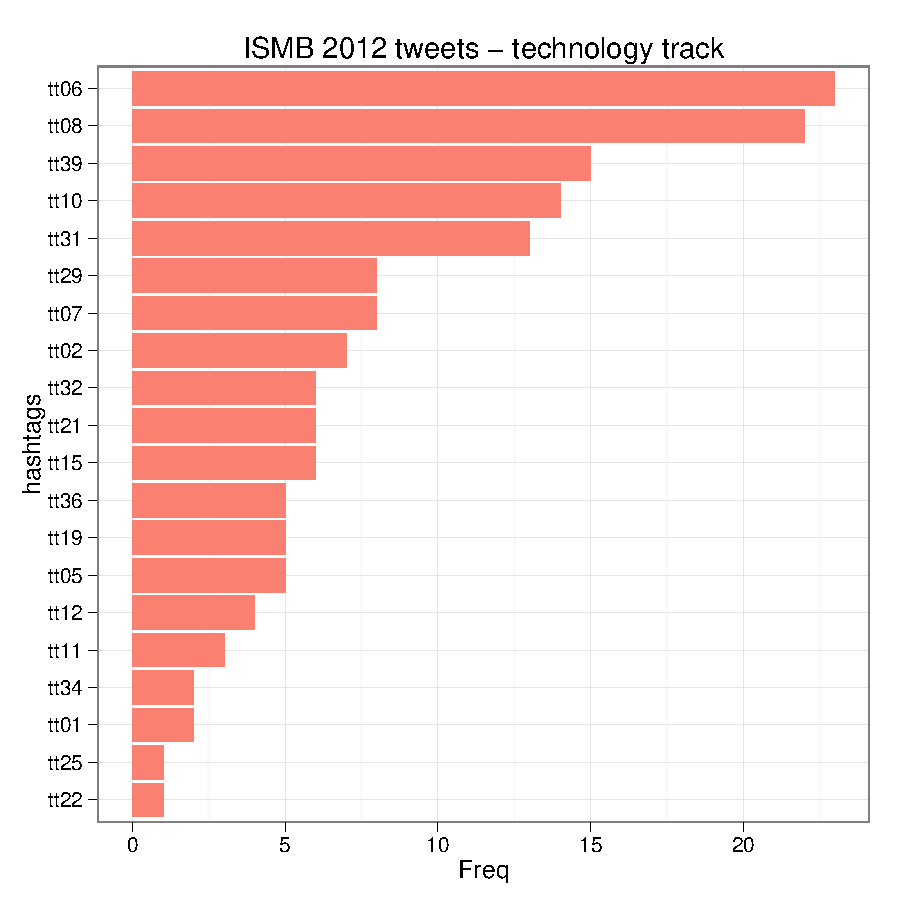
\includegraphics{ismb-008}
\end{center}

TT06: The Taverna Server - Executing Scientific Workflows Remotely (Katy Wolstencroft).

\newpage

\subsection{Workshops}
\begin{center}
\begin{Schunk}
\begin{Sinput}
> wk <- ht[grep("^wk", ht$hashtags),]
> wk$hashtags <- factor(wk$hashtags, levels = as.character(wk$hashtags))
> print(ggplot(wk) + geom_bar(aes(hashtags, Freq), fill = "salmon") + 
+   coord_flip() + theme_bw() + opts(title = "ISMB 2012 tweets - workshops"))
\end{Sinput}
\end{Schunk}
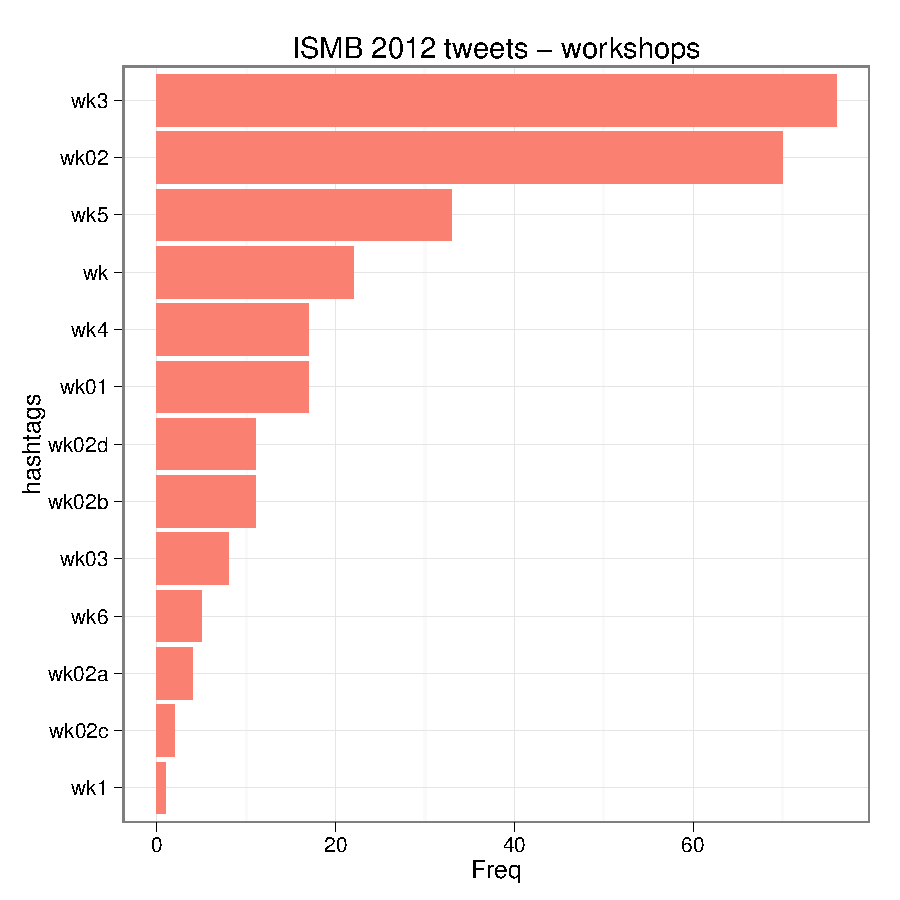
\includegraphics{ismb-009}
\end{center}

WK 3: Bioinformatics Core Facilities (Simon Andrews, Fran Lewitter, Brent Richter, David Sexton).

\newpage

\section{Users}
\subsection{The long tail}
\begin{center}
\begin{Schunk}
\begin{Sinput}
> users <- as.data.frame(table(ismb$screenName))
> colnames(users) <- c("user", "tweets")
> users <- users[sort.list(users$tweets, decreasing = T),]
> print(ggplot(users) + geom_point(aes(1:nrow(users), tweets), color = "salmon") + theme_bw() + 
+   opts(title = "ISMB 2012 tweets per user") + xlab("User"))
\end{Sinput}
\end{Schunk}
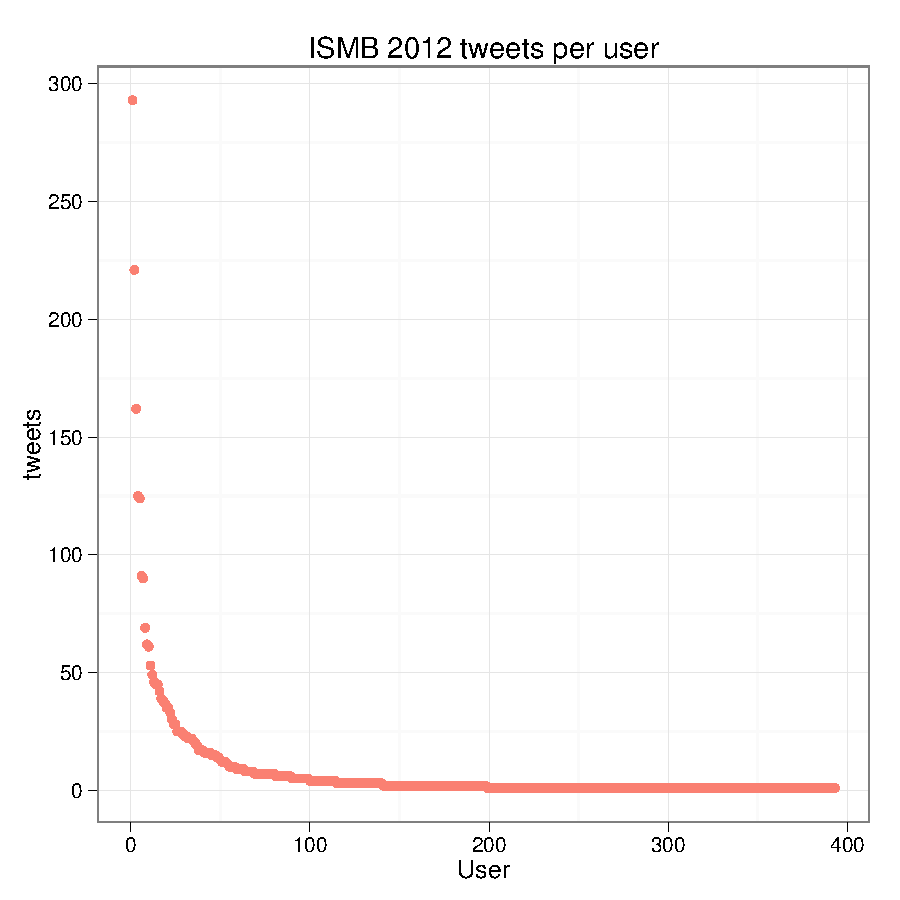
\includegraphics{ismb-010}
\end{center}

\subsection{The top 10}
% latex table generated in R 2.15.1 by xtable 1.7-0 package
% Thu Aug 23 13:35:01 2012
\begin{table}[ht]
\begin{center}
\begin{tabular}{lr}
  \hline
user & tweets \\ 
  \hline
Chris\_Evelo & 293 \\ 
  genetics\_blog & 221 \\ 
  tladeras & 162 \\ 
  iGenomics & 125 \\ 
  WonderMixTape & 124 \\ 
  alexishkin &  91 \\ 
  bffo &  90 \\ 
  spitshine &  69 \\ 
  Albertagael &  62 \\ 
  andrewsu &  61 \\ 
   \hline
\end{tabular}
\caption{Most tweets - top 10 users}
\end{center}
\end{table}
\newpage

\section{Text mining}
\subsection{Word frequency}
First, get all words composed only of alphanumeric characters.
\begin{Schunk}
\begin{Sinput}
> sw    <- stopwords("en")
> words <- lapply(words, function(x) x[grep("^[A-Za-z0-9]+$", x)])
> words <- unlist(words)
> words <- tolower(words)
> words <- words[-grep("^[rm]t$", words)]
> words <- words[!words %in% sw]
> words.t <- as.data.frame(table(words))
> words.t <- words.t[sort.list(words.t$Freq, decreasing = T),]
> print(xtable(head(words.t, 10), caption = "Top 10 words in tweets"), include.rownames = FALSE)
\end{Sinput}
% latex table generated in R 2.15.1 by xtable 1.7-0 package
% Thu Aug 23 13:35:02 2012
\begin{table}[ht]
\begin{center}
\begin{tabular}{lr}
  \hline
words & Freq \\ 
  \hline
data & 251 \\ 
  talk & 238 \\ 
  using & 132 \\ 
  gene & 117 \\ 
  protein &  80 \\ 
  slides &  73 \\ 
  network &  71 \\ 
  people &  69 \\ 
  analysis &  68 \\ 
  ismb &  66 \\ 
   \hline
\end{tabular}
\caption{Top 10 words in tweets}
\end{center}
\end{table}\end{Schunk}

\setkeys{Gin}{width=0.6\textwidth}
\begin{center}
\begin{Schunk}
\begin{Sinput}
> pal2 <- brewer.pal(8, "Dark2")
> wordcloud(words.t$words, words.t$Freq, scale = c(8, .2), min.freq = 3,
+     max.words = 200, random.order = FALSE, rot.per = .15, colors = pal2)
\end{Sinput}
\end{Schunk}
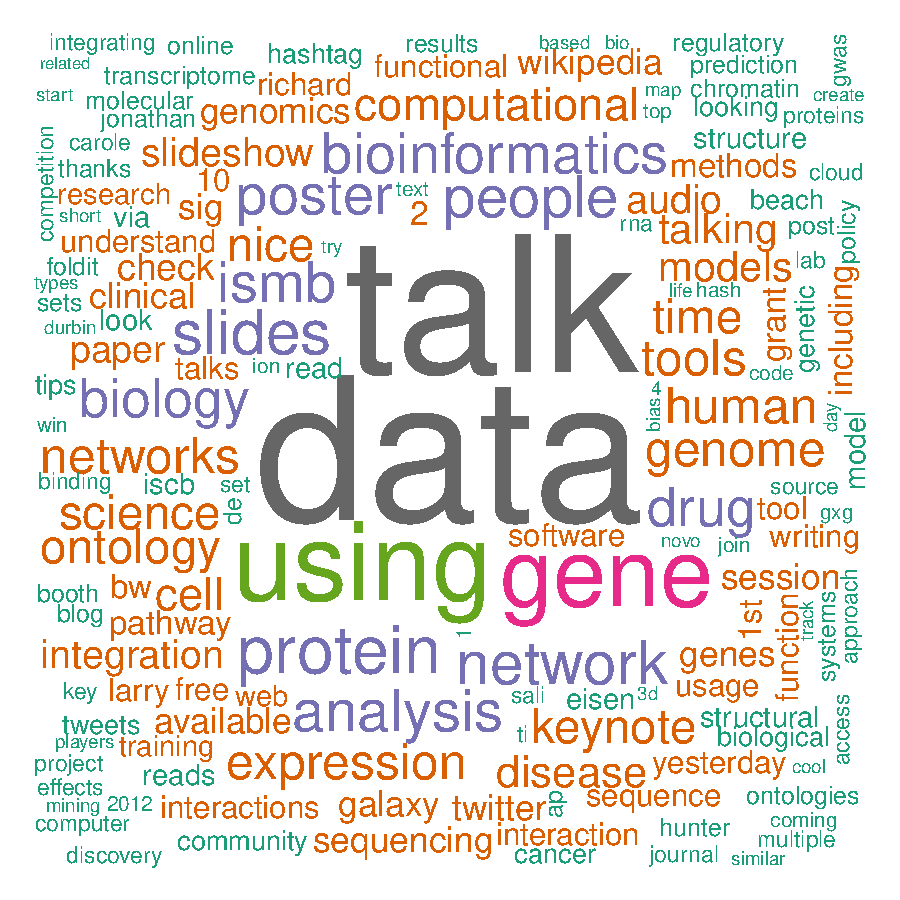
\includegraphics{ismb-013}
\end{center}

\newpage

\subsection{Sentiment analysis}

\subsubsection{Emotions}
\begin{Schunk}
\begin{Sinput}
> em <- classify_emotion(ismb$text, algorithm = "bayes")
> print(xtable(table(em[, "BEST_FIT"]), caption = "Tweet emotion"))
\end{Sinput}
% latex table generated in R 2.15.1 by xtable 1.7-0 package
% Thu Aug 23 13:36:39 2012
\begin{table}[ht]
\begin{center}
\begin{tabular}{rr}
  \hline
 & V1 \\ 
  \hline
anger &  24 \\ 
  disgust &   4 \\ 
  fear &  11 \\ 
  joy & 149 \\ 
  sadness &  44 \\ 
  surprise &  37 \\ 
   \hline
\end{tabular}
\caption{Tweet emotion}
\end{center}
\end{table}\end{Schunk}

Shall we look at a "joyous" tweet?

\begin{lstlisting}
Hooray! First #comicsans talk of the conference. Didn't take long. It's like an old friend that refuses to die. #ismb
\end{lstlisting}

\subsubsection{Polarity}
\begin{Schunk}
\begin{Sinput}
> po <- classify_polarity(ismb$text, algorithm = "bayes")
> print(xtable(table(po[, "BEST_FIT"]), caption = "Tweet polarity"))
\end{Sinput}
% latex table generated in R 2.15.1 by xtable 1.7-0 package
% Thu Aug 23 13:37:09 2012
\begin{table}[ht]
\begin{center}
\begin{tabular}{rr}
  \hline
 & V1 \\ 
  \hline
negative & 573 \\ 
  neutral & 197 \\ 
  positive & 2392 \\ 
   \hline
\end{tabular}
\caption{Tweet polarity}
\end{center}
\end{table}\end{Schunk}

A "positive" tweet:
\begin{lstlisting}
Often forgotten: CS Optimizing (network) models only makes sense when you keep the model simple to not overfit #ISMB #netbiosiig
\end{lstlisting}

A "negative" tweet:
\begin{lstlisting}
Chris Sander in Network Biology SIG and how translational medicine: tries to explain how complicated it all is in cancer biology #ISMB
\end{lstlisting}

\end{document}
